\newpage 
\thispagestyle{empty}
\chapter{Implementierung}\label{sec:Implementierung}
Wie im Kapitel \ref{sec:Interpretation_Dipol} erwähnt, wird die Antennenstruktur weder auf einer FR4 Kunstharzplatte noch auf eine Plastikfolie aufgedruckt, da einerseits die Produktionskosten von Kleinserien im Verhältnis zum Nutzen eher gross sind, und weil andererseits, jeder Fertigungsdurchgang von gedruckten Antennen mindestens ein bis drei Tage benötigt. Daher werden die zu testenden Antennen aus einer Kupferfolie geschnitten. So können Änderungen im Designs sehr schnell umgesetzt werden und die Kosten sind gering.\\

Aus der Interpretation der Dipolantennen Simulationen im Kapitel ( \ref{sec:Interpretation_Dipol}) ist hervorgegangen, dass das Abstrahlverhalten einer Dipolantenne mit einer Breite von 3 mm und einer Dicke von 26 $\mu m$ sowie der Länge von 50.25 mm ausgemessen wird. Wie die Abbildung \ref{S11_Vergleich_Simulation_Dipolantenn_freiraum_Geraet} zeigt, unterscheidet sich das Abstrahlverhalten von Dipole mit einer Breite von 1 mm und 3 mm nur unwesentlich. Die Antennenstruktur mit einer Breite von 3 mm ist wesentlich einfacher zu bearbeiten als die 1 mm Breiten Antennenstruktur. Das Kupferband mit einer Breite von weniger als 3 mm kann unter geringem Zug reissen. Zudem ist die grössere Fläche mit Klebstoff von Vorteil um die Antenne an das Kunststoffgehäuse zu fixieren.  \\

Die Antenne wird mit dem Skalpell aus dem Kupferklebeband ausgeschnitten. Das ist in der Abbildung \ref{fig:DipolausKupferband} gezeigt. Dabei gilt es zu beachten, dass sich das Kupferband nicht in seine ursprünglicher Form zurück zieht. Das Zentrum der Antenne, dient als Fusspunkt der Antenne, dieser wird mit einem ca. 1 mm$^{2}$ grosssen Lötzinnpunkt versehen. An diesem speist die Zuleitung, in Form eines Koaxialkabels, die Antenne.\\
\begin{figure}[!ht]
	\centering
	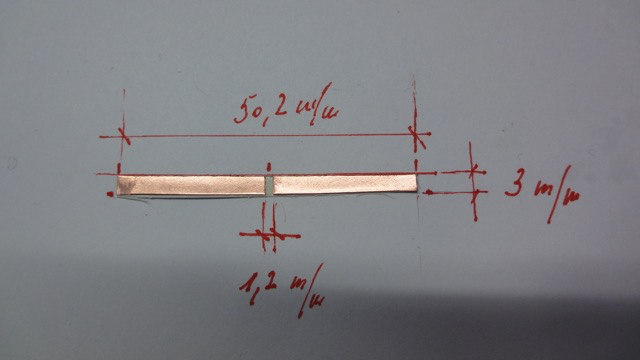
\includegraphics[width=13cm]{content/bilder/Implementierung/Dipol3mm50mm.jpg}%
	\caption{Dipol aus Kupferklebeband ausgeschnitten}
	\label{fig:DipolausKupferband}
\end{figure}
%\newpage

In der Abbildung \ref{fig:DipolausKupferbandGeraeteinnenseite} ist  die Dipolantenne mit einem Koaxialkabel als Speiseleitung gezeigt. Das Koaxialkabel dient als längs homogene Leitung. Sie führt die elektromagnetische Welle von der Quelle zur Antenne. Die Leitung wird rechtwinklig von der Antenne weggeführt. Es muss stehst darauf geachtet werden, dass sich das der Biegeradius des Koaxialkabels eingehalten wird. Der Aussenleiter des Koaxialkabels muss nicht zusätzlich gegenüber dem darunterliegenden Akkupaket isoliert werden. Denn dieser ist bereits in eine Kunststofffolie gehüllt. Jedoch muss darauf geachtet werden, dass der Aussenleiter des Koaxialkabels, nicht mir der Elektronikplatine, die sich auf der Rückseite des Displays befindet, kurzschliesst. Daher erfüllt das Papierklebeband mehrere Aufgaben. Es dient als Isolation zwischen der Elektronikplatine und dem Koaxialkabel und zusätzlich als Zugsentlastung der Antenne. Des weitern hilft das Papierklebeband zur Fixierung der Antenne.\\
\begin{figure}[!ht]
	\centering
	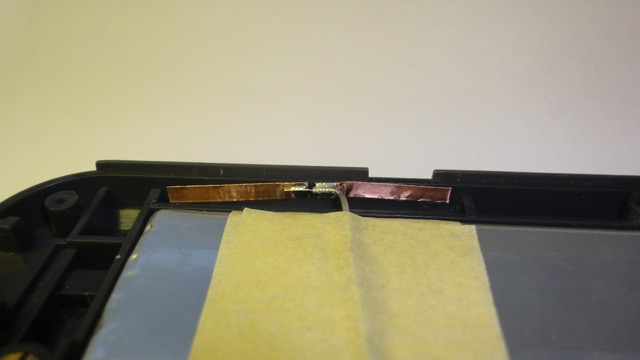
\includegraphics[width=13cm]{content/bilder/Implementierung/DipolIMGeraet.jpg}%
	\caption{Dipol aus Kupferklebeband an der Geräteinnenseite befestigt}
	\label{fig:DipolausKupferbandGeraeteinnenseite}
\end{figure}

\newpage
Die Abbildung \ref{fig:DipolimGeraet} zeigt, wie die Antenne im Fluginstrumet positioniert ist. Auf dieser Abbildung ist sehr gut zu erkennen, dass die Antenne direkt an die Aussenwand Kunststoffgehäuse des Kuststoffgehäuse des Fluginstumetes geklebt ist. Das Koaxialkabel führt rechtwinklig von der Antenne weg. Bis zum SMA Stecker, über diesen wird die Antenne mit der interne Quelle des StarLab verbunden.\\
\begin{figure}[!ht]
	\centering
	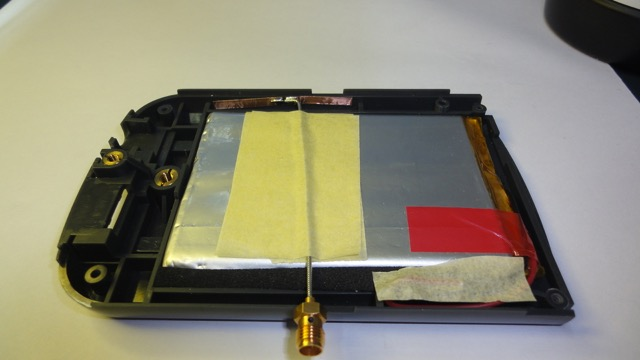
\includegraphics[width=13cm]{content/bilder/Implementierung/DipolKabelGeraet.jpg}%
	\caption{Dipol im Gerät und Koaxialkabel}
	\label{fig:DipolimGeraet}
\end{figure}






